\chapter{Detalhes da Implementação}

\section{Introdução}
\label{sec:Detalhes da Implementação}

Este capítulo detalha a implementação do sistema de treinamento e inserção automática desenvolvido para a geração de ambientes virtuais a partir de imagens. A aplicação foi concebida para automatizar o processo de geração de modelos tridimensionais a partir das imagens processadas. O objetivo principal da implementação é oferecer uma solução eficiente para qualquer usuário que deseja criar ambientes virtuais, possa fazê-lo de maneira rápida e intuitiva, com base em imagens fornecidas.

A aplicação, desenvolvida dentro da plataforma Unity, permite ao usuário carregar imagens através de um menu gráfico e, a partir delas, o sistema realiza automaticamente o reconhecimento dos objetos presentes dentro da foto fornecida e os insere no ambiente virtual. Essa abordagem reduz significativamente a necessidade de intervenção manual, tornando o processo de criação de ambientes 3D mais eficiente. A automação deste processo é particularmente útil para usuários com pouca experiência técnica na geração de ambientes virtuais, permitindo-lhes focar na interatividade do ambiente ambiente sem se preocupar com os detalhes gráficos.


\section{Estrutura geral da aplicação}

A estrutura da aplicação desenvolvida neste trabalho está representada na Figura \ref{fig:estrutura}. A arquitetura do sistema é composta por quatro elementos principais que operam em conjunto para realizar a tarefa de criação de ambientes virtuais. O fluxo do processo inicia-se com o treinamento do modelo YOLO, que gera os pesos da RNC utilizados no reconhecimento de objetos nas imagens fornecidas.

\begin{figure}[!h]
    \centering
    \begin{minipage}{1\linewidth}
    \centering
    \captionsetup{justification=centering,margin=0.5cm,font=small}
    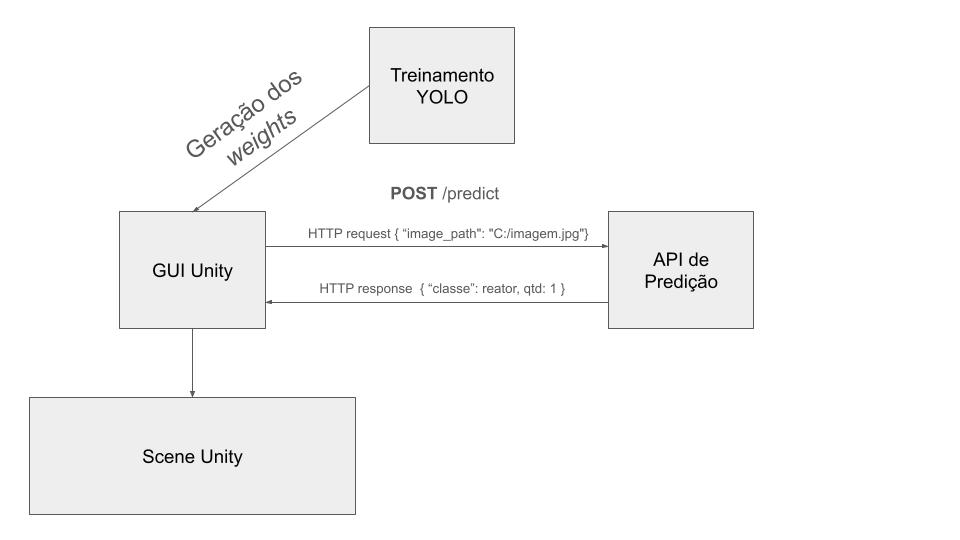
\includegraphics[width=1\linewidth]{img/cap5/estrutura.jpg}
    \caption{Estrutura geral da Aplicação}.
    \label{fig:estrutura}
    \end{minipage}
\end{figure}

O segundo componente importante da estrutura é a interface gráfica do usuário (\textit{Graphical User Interface} - GUI) no Unity, que pode ser visualizada na Figura \ref{fig:GUI}. Esta interface foi cuidadosamente projetada para facilitar a identificação e modelagem das cenas virtuais. O script que compõe a GUI é integrado diretamente ao Unity, proporcionando ao usuário uma ferramenta intuitiva para selecionar imagens e iniciar o processo de reconhecimento. A GUI comunica-se com uma \textit{API} que aplica o modelo treinado às imagens fornecidas, enviando uma requisição \textit{HTTP} com os dados necessários

Conforme ilustrado no diagrama, a \textit{API} recebe o caminho da imagem, aplica os pesos treinados da RNC, e retorna ao Unity a quantidade de objetos identificados e suas respectivas classes. No caso, o protótipo foi desenvolvido para trabalhar com apenas uma classe, abrindo espaço para trabalhos futuros, assim como ele também não implementa a localização espacial dos objetos, os modelos virtuais gerados são dispostos de forma uniforme na cena do Unity após o processamento da imagem. Isso significa que, apesar da precisão na detecção dos objetos, ainda há espaço para melhorias no que diz respeito à colocação exata dos modelos dentro do ambiente virtual, o que será uma possível melhoria em versões futuras do sistema.

\begin{figure}[!h]
    \centering
    \begin{minipage}{0.7\linewidth}
        \centering
        \captionsetup{justification=centering,margin=0.5cm,font=small}
        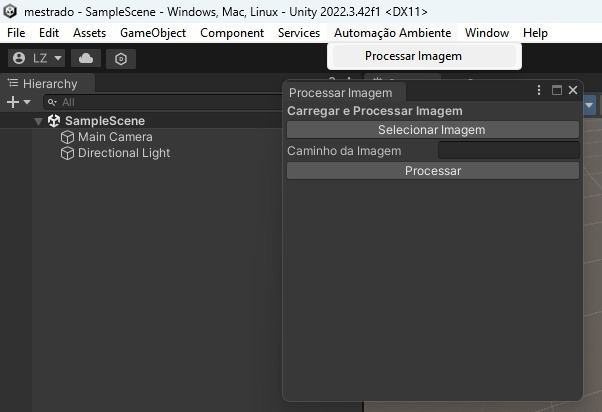
\includegraphics[width=\linewidth]{img/cap5/GUI-TOOL.jpeg}
        \caption{Interface para o usuário.}
        \label{fig:GUI}
    \end{minipage}
\end{figure}

\section{Treinamento com a YOLO}

O treinamento com o YOLO segue um padrão comum entre suas diferentes versões, mas cada versão possui características específicas em termos de pacotes necessários e processos de instalação. 

\subsection{Treinamento com a YOLOv5, YOLOv6 e YOLOv8}

A YOLOv5\footnote{\url{https://github.com/ultralytics/yolov5}}, assim como a YOLOv6\footnote{\url{https://github.com/meituan/YOLOv6}} e a YOLOv8\footnote{\url{https://github.com/ultralytics/ultralytics}}, foram desenvolvidas pela empresa \textit{Ultralytics}, que também dá nome à biblioteca utilizada para a configuração do projeto. Para utilizar essa versão da arquitetura, foi necessário clonar o projeto para a máquina onde o treinamento foi executado. Além disso, foi utilizada a versão 3.1 do \textit{Python}.

Em aplicações desenvolvidas em \textit{Python}, é altamente recomendada a criação de um ambiente virtual para garantir que as bibliotecas sejam instaladas corretamente e que o ambiente não entre em conflito com outras dependências do sistema. Esse ambiente virtual isola o projeto e suas dependências de outros projetos e bibliotecas instaladas globalmente. As dependências necessárias para o projeto estão especificadas no arquivo \textit{requirements.txt}.

Para configurar o ambiente virtual e instalar as dependências, foram executados no terminal dentro da pasta do projeto os seguintes comandos:

\begin{lstlisting}
python -m venv ambiente_virtual
.\ambiente_virtual\Scripts\activate
pip install -r requirements.txt
\end{lstlisting}

Após isso, foi desenvolvido a estrutura básica do script de treinamento de todas essas versões da YOLO. A Figura \ref{fig:script-yolov5-6} apresenta os scripts para o treinamento da YOLOv5, na imagem superior, e YOLOv6 na imagem inferior. Basicamente, a primeira linha designa a importação da biblioteca da \textit{Ultralytics}. Logo em seguida, é especificado a arquitetura que será utilizada. Para a quinta versão, foi designado \textit{‘YOLOv5n.pt’}; para sexta versão, foi especificado \textit{‘YOLOv5n.pt’}. A última linha por fim, determina a modelagem do treinamento, que será especificada na função \textit{train()}, do objeto \textit{model}, do tipo \textit{YOLO()}. Foram especificados três parâmetros diferentes. O primeiro, \textit{data} recebe o arquivo de configuração \textit{"config.yaml"}, em que é especificado a quantidade de classes a serem treinadas (neste caso, apenas uma, que é a classe "reator"), e a localização dos diretórios contendo as imagens e marcações para treinamento, validação e teste. Em seguida, há o parâmetro \textit{epochs}, que configura a quantidade de iterações que a RNC irá realizar. Neste caso, foi configurado para 300 iterações. O parâmetro \textit{batch}, naturalmente, configura o valor de \textit{batch}, que foi variado de 2 a 16. Por fim, \textit{optimizer} determina o otimizador, que na comparação inicial foi utilizado no valor de ‘SGD’, aplicando o otimizador homônimo. 

\begin{figure}[!h]
    \centering
    \begin{minipage}[b]{0.49\linewidth}
        \centering
        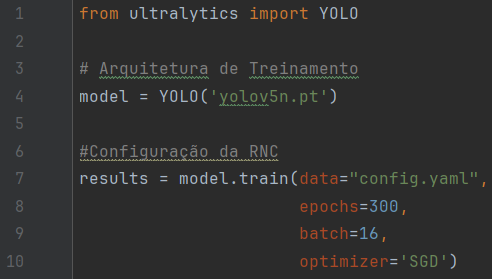
\includegraphics[width=1\linewidth]{img/cap5/script-yolov5.png}
    \end{minipage}
    \hspace{0.05\linewidth}
    \begin{minipage}[b]{0.49\linewidth}
        \centering
        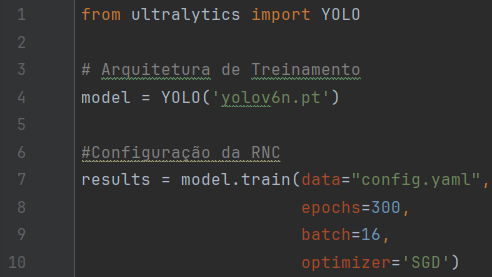
\includegraphics[width=1\linewidth]{img/cap5/script-yolov6.png}
    \end{minipage}
    \captionsetup{justification=centering,margin=0.5cm,font=small}
    \caption{Demonstração dos Scripts de Treinamento das versões YOLOv5, em cima, e YOLOv6, em baixo.}
    \label{fig:script-yolov5-6}
\end{figure}

\subsection{Treinamento com a YOLOv7}

De todas as versões da YOLO, apenas a YOLOv7\footnote{\url{https://github.com/WongKinYiu/yolov7}} foi executada via terminal. Todo o preparo do ambiente foi igual às demais versões. Fez-se a cópia do repositório remoto no computador que a executou, utilizou-se a mesma versão do \textit{Pyhton}, e foi gerado um ambiente virtual para aquisição das dependências. Dentro do diretório da YOLOv7, ao contrário de executar um \textit{script} por meio de um ambiente de desenvolvimento, fez a execução do comando demonstrado na Figura \ref{fig:script-yolov7}, diretamente via terminal. O início da instrução se inicia com \textit{python}, para indicar qual o tipo de aplicação executada. Em seguida, é especificado o arquivo da classe \textit{train.py}, que é a responsável por toda estruturação do treinamento da RNC.  A parametrização é semelhante às demais, com \textit{batch-size} determinando o valor de \textit{batch}; \textit{epochs}, épocas; e \textit{data}, a configuração das classes e diretórios das imagens; \textit{weights}, indicando a arquitetura utilizada que seria \textit{‘yolov7.pt’}. Diferindo das outras, há a especificação do tipo de processador por meio de \textit{device}, que no caso foi escolhido CPU.

\begin{figure}[!h]
    \centering
    \begin{minipage}{0.7\linewidth}
    \centering
    \captionsetup{justification=centering,margin=0.5cm,font=small}
    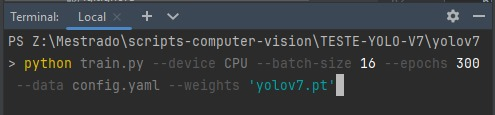
\includegraphics[width=1\linewidth]{img/cap5/script-yolov7.jpg}
    \caption{Comando de Execução da YOLOv7}.
    \label{fig:script-yolov7}
    \end{minipage}
\end{figure}

\subsection{Variação dos otimizadores com a YOLOv8}

Seguindo a mesma metodologia empregada no trabalho de \cite{gonzaga2023identificaccao}, foi variado o parâmetro referente ao otimizador. A estrutura do treinamento é igual à anteriormente referida para essa versão, apenas o valor do parâmetro do otimizador que será alterado. Os testes com o otimizador Adam, receberam a configuração \textit{optimizer=’Adam’}, para Adam; \textit{optimizer=’AdamW’}, para AdamW; e \textit{optimizer=’SGD’} para SGD. Na Figura \ref{fig:script-yolov8} é demonstrado a configuração desse treinamento.

\begin{figure}[!h]
    \centering
    \begin{minipage}{0.7\linewidth}
    \centering
    \captionsetup{justification=centering,margin=0.5cm,font=small}
    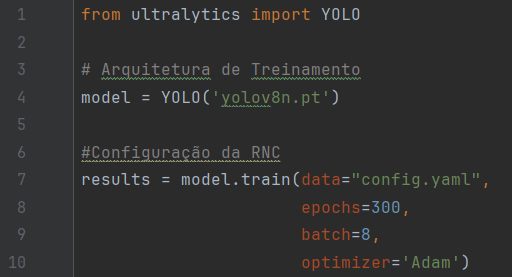
\includegraphics[width=1\linewidth]{img/cap5/yolov8-adam.png}
    \caption{Demonstração do Script de Treinamento da YOLOv8, com aplicação do otimizador Adam e com \textit{batch} configurado para 8}.
    \label{fig:script-yolov8}
    \end{minipage}
\end{figure}

Diferentemente dos demais, a fim de avaliar a melhor configuração da YOLOv8, para cada variação do otimizador foi realizado a variação do \textit{batch}, nos valores de 2, 4, 8 e 16. Com isso, pode-se comparar o efeito dos otimizadores e tamanho de lote nas diversas configurações dessa arquitetura.

\section{API de Identificação}

A construção da aplicação responsável pelo processamento das imagens enviadas pela Unity envolveu a criação de um \textit{endpoint} que permite a solicitação do serviço de processamento por aplicações externas. Sua estrutura é demonstrada na \ref{fig:api-identificacao}. O Unity envia uma requisição \textit{HTTP} para o endereço \textit{"localhost:5000/predict"}, incluindo o caminho da imagem no corpo da requisição. Ao receber a requisição, o \textit{endpoint} decodifica seu corpo para extrair o endereço da localização da imagem a ser processada, que será armazenado na variável \textit{imagePath}. Na linha seguinte, tem-se a atribuição \textit{model = YOLO(‘best.pt’)}. O O arquivo \textit{best.pt} carrega as informações relativas ao melhor treinamento da experimentação para ser aplicado no processo de predição. Na linha seguinte, aplica-se os pesos responsáveis pela predição à imagem especificada no caminho. Realizado esse processo, a iteração que é feita logo após, trata de extrair do arquivo resultante a localização de cada reator identificado. Passa-se essa informação por coordenadas de \textit{bounding box}, idênticas ao processo de marcação. Além de poder contabilizar a quantidade de reatores detectados, é possível localizar visualmente os objetos detectados na foto processada.

\begin{figure}[!h]
    \centering
    \begin{minipage}{0.7\linewidth}
    \centering
    \captionsetup{justification=centering,margin=0.5cm,font=small}
    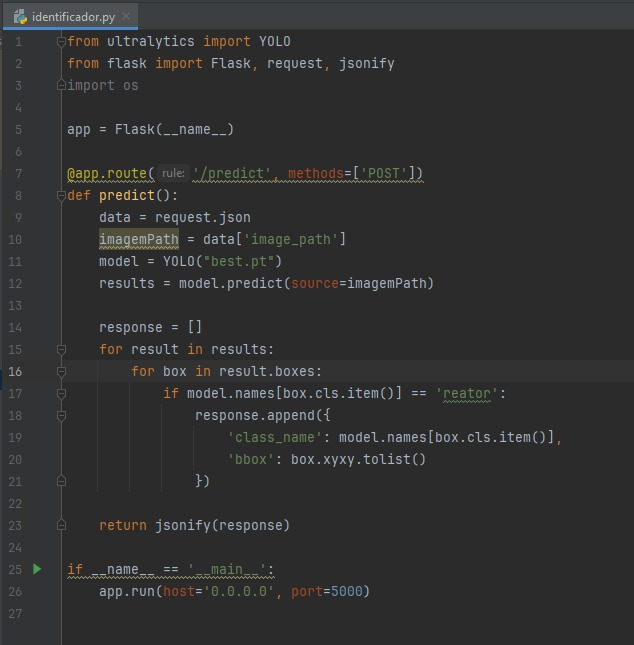
\includegraphics[width=1\linewidth]{img/cap5/API.jpeg}
    \caption{\textit{API} de identificação de imagem}.
    \label{fig:api-identificacao}
    \end{minipage}
\end{figure}

Para executar esta aplicação, você precisará do Python 3.5 ou superior instalado em seu sistema. Pode-se instalar as dependências manualmente usando o comando \textit{pip install}, especificando os pacotes necessários. Neste caso, como o script utiliza Flask e o YOLO da biblioteca \textit{Ultralytics}, pode-se instalar essas bibliotecas com o seguinte comando: \textit{pip install flask ultralytics}. Após instalar as dependências, supondo que o script seja salvo em um arquivo chamado \textit{api-rv.py}, abra um terminal no diretório onde o script está localizado e execute o comando: \textit{python api-rv.py}. Isso iniciará o servidor Flask e tornará o endpoint \textit{"/predict"} acessível para aplicações externas, como o Unity. O código completo do script \textit{api-rv.py} está localizado no Apêndice A.

\subsection{Implementação na Unity}

O script desenvolvido no Unity é dividido em alguns métodos. Inicialmente, há a disposição na tela da interface gráfica, representada na Figura \ref{fig:metodo-gui}. Este código define o nome da janela, suas dimensões e os tipos de interações que o usuário pode realizar, como selecionar uma imagem e iniciar o processamento. A GUI foi desenvolvida com foco na usabilidade, garantindo que até mesmo usuários com pouca experiência em Unity possam operar a implementação com facilidade. O código completo que habilita esta implementação dentro do Unity, entitulado \textit{ModelLoaderMenu.cs}, está localizado no Apêndice B. Copiá-lo em um arquivo homônimo e colocá-lo dentro do projeto Unity é suficiente para poder utilizá-lo.

\begin{figure}[!h]
    \centering
    \begin{minipage}{0.7\linewidth}
    \centering
    \captionsetup{justification=centering,margin=0.5cm,font=small}
    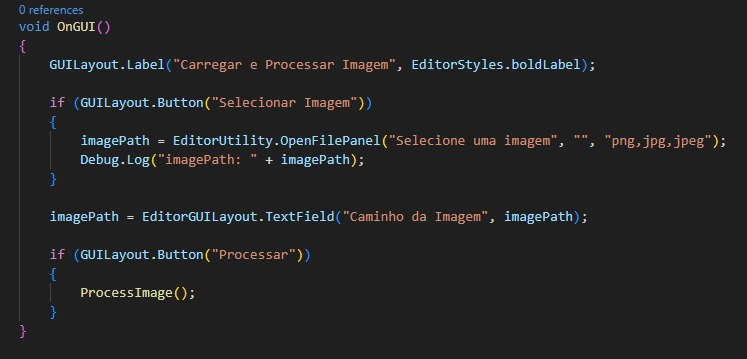
\includegraphics[width=1\linewidth]{img/cap5/gui-codigo.jpeg}
    \caption{\textit{API} de identificação de imagem}.
    \label{fig:metodo-gui}
    \end{minipage}
\end{figure}

Ao pressionar o botão de processamento, o método correspondente é ativado, conforme ilustrado na Figura \ref{fig:metodo-disposicao}. Este método chama outro, que é responsável por enviar a requisição \textit{HTTP} para a \textit{API} processar a resposta recebida. Com as informações retornadas pela \textit{API}, o \textit{script} percorre cada objeto identificado e o insere na cena do Unity, posicionando-os de acordo com uma disposição pré-definida. 

É importante destacar que o modelo tridimensionald o reator, nesta aplicação, foi armazenado dentro do próprio diretório do projeto, e é armazenado e uma variável \textit{modelPath} conforme a linha:

\begin{lstlisting}
string modelPath = "Assets/Model/FILTER_F10.fbx";
\end{lstlisting}

Naturalmente, em uma expansão deste protótipo, seria possível uma integração da aplicação com um sistema de armazenamento remoto, haja visto que a coleção da modelagem de diversos equipamentos pode ser custosa em termos de armazenamento, assim como possibilitaria um desacoplamento da API com seus componentes. A computação em nuvem, que é entendida como um modelo de entrega de serviços que permite o acesso sob demanda a recursos computacionais compartilhados, como servidores, armazenamento e redes, pode ser uma solução viável para esse tipo de expansão \cite{mell2011nist}. Este modelo permitiria o armazenamento e a gestão eficiente de modelos tridimensionais, ao mesmo tempo que possibilitaria escalabilidade e flexibilidade à medida que a coleção de modelos cresce, sem sobrecarregar os recursos locais.

\begin{figure}[!h]
    \centering
    \begin{minipage}{0.7\linewidth}
    \centering
    \captionsetup{justification=centering,margin=0.5cm,font=small}
    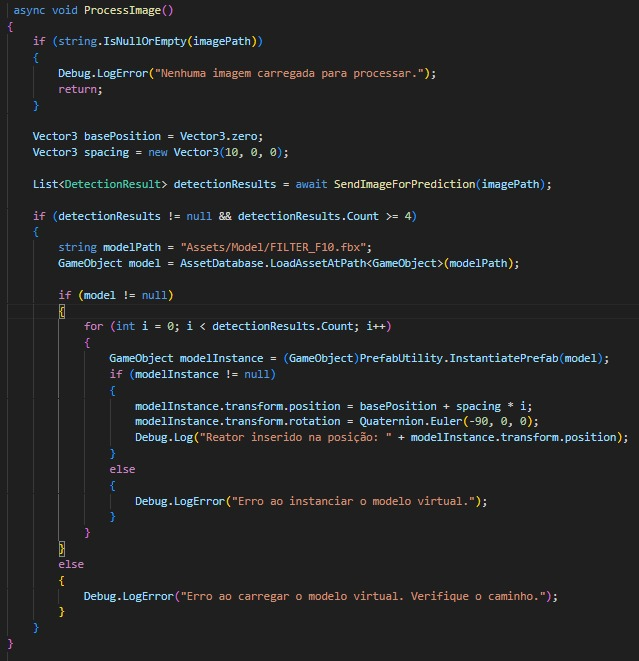
\includegraphics[width=1\linewidth]{img/cap5/process-image.jpeg}
    \caption{Método de processamento da imagem e inserção dos modelos conforme a resposta da \textit{API}}.
    \label{fig:metodo-disposicao}
    \end{minipage}
\end{figure}

Após o processamento da imagem, o número de reatores identificados pelo modelo é automaticamente renderizado na cena do Unity. Essa etapa garante que os objetos reconhecidos sejam visualmente representados no ambiente virtual, facilitando a interação e análise do usuário. Neste protótipo, os reatores identificados são posicionados com espaçamento padrão entre um e outro. Não há um posicionamento correto dos equipamentos, sendo esta uma demanda para implementações futuras. A Figura \ref{fig:predict} ilustra um exemplo de imagem processada, na qual foram corretamente identificados e inseridos quatro reatores na cena. A quantidade de reatores e outros objetos detectados e inseridos na cena depende diretamente da precisão do modelo de reconhecimento utilizado, bem como da qualidade e clareza dos elementos presentes na imagem original. Dessa forma, um modelo bem treinado, aliado a uma imagem nítida e bem enquadrada, resulta em uma identificação mais precisa e uma correspondência fiel entre os objetos detectados e os inseridos no ambiente virtual. Esse processo automatizado não apenas melhora a eficiência da criação de cenas no Unity, mas também minimiza a necessidade de ajustes manuais, proporcionando uma experiência mais fluida e prática para o usuário.

\begin{figure}[!h]
    \centering
    \begin{minipage}{0.9\linewidth}
    \centering
    \captionsetup{justification=centering,margin=0.5cm,font=small}
    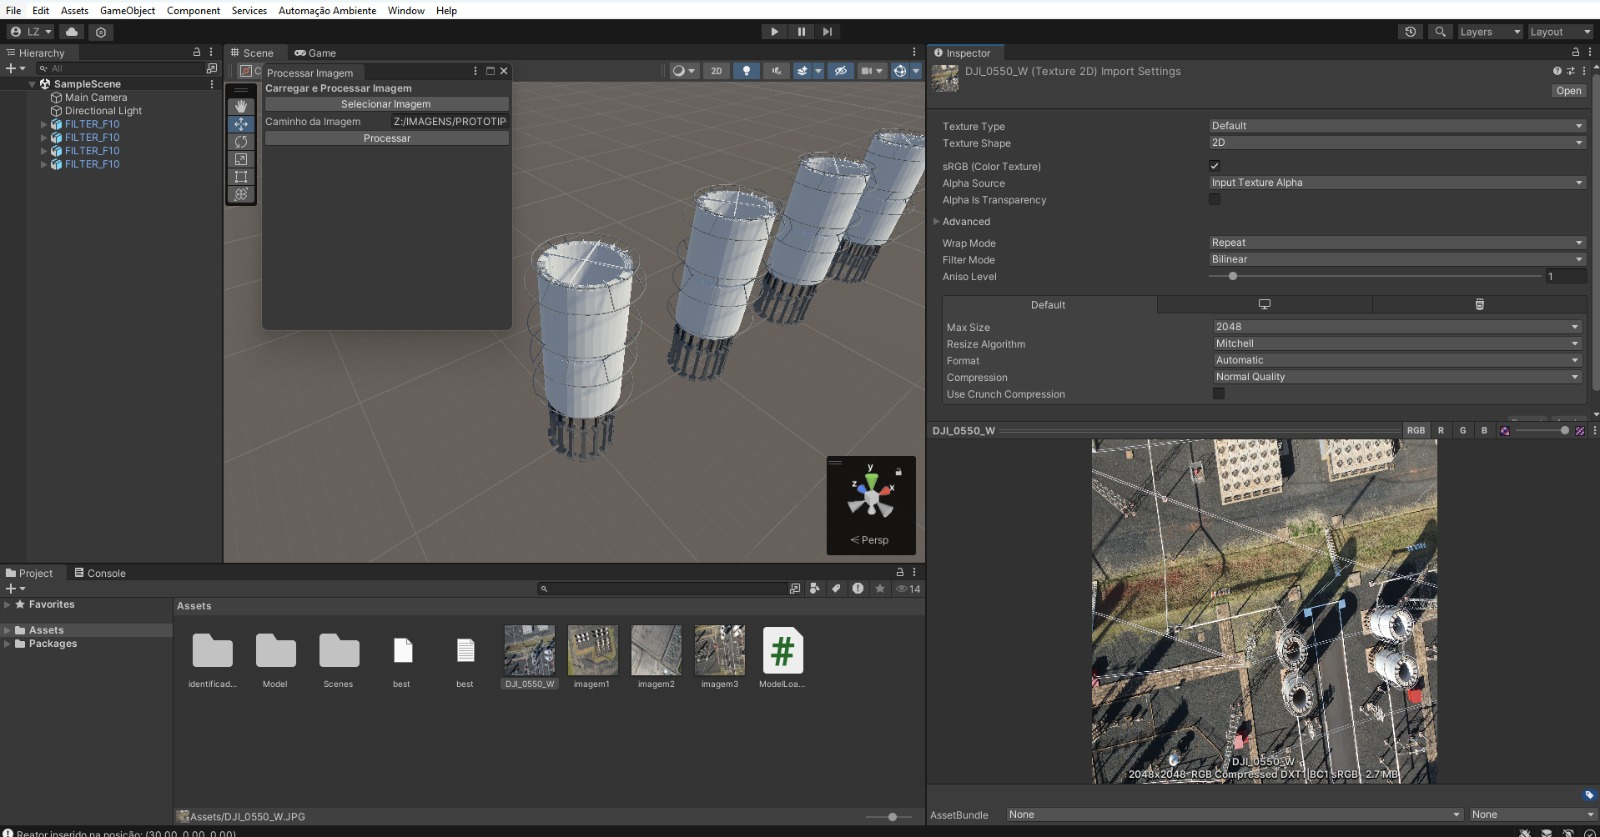
\includegraphics[width=1\linewidth]{img/cap5/predict.jpeg}
    \caption{Método de processamento da imagem e inserção dos modelos conforme a resposta da \textit{API}}.
    \label{fig:predict}
    \end{minipage}
\end{figure}

\section{Conclusão}

A implementação desenvolvida é altamente intuitiva e de fácil utilização. Para executá-la em um computador pessoal, basta inserir o script direcionado para o Unity dentro do projeto e, em paralelo, rodar o código da \textit{API} em um arquivo separado. Essa aplicação se destaca como uma solução prática e eficiente, oferecendo um método simplificado que pode gerar um impacto significativo no desenvolvimento de ambientes de RV.


	











